\documentclass[12pt]{article}
\usepackage[margin=1in]{geometry}
\usepackage{graphicx}
\graphicspath{ {images/} }
\usepackage{fontspec}
\setmainfont[Path=/usr/share/fonts/truetype/calibri/,
    BoldItalicFont=CALIBRIZ.ttf,
    BoldFont      =CALIBRIB.ttf,
    ItalicFont    =CALIBRII.ttf]{Calibri.ttf}
\title{Lab 04: Friction}
\author{Adris Jautakas, partnered with Matthew Kendall}
\date{January 22, 2018}
\begin{document}
    \maketitle

    \pagebreak

    \section*{Abstract}
        \begin{quote}
        {\textit {\small 
            The following lab investigates friction through a series of tests 
            involving sliding blocks against a surface. We evaluated how 
            friction is proportionally dependent on its normal force, and how
            the friction coefficients $\mu_s$ and $\mu_k$ can be determined
            and evaluated in such a system.
        } }
        \end{quote}

    \section{Introduction}
        \par When matter physically interacts with other matter, the resistance
        that the matter faces is what's known as Friction. When two surfaces rub 
        against each other, their edges are always imperfect and bumpy, which 
        causes the surfaces to push back against their movement from their 
        friction. This frictional force is directly proportional to the pressure
        between the objects, and varies depending on the type of material. An
        equation to determine the frictional force of two surfaces relies on
        these principles, which states that $F_{fric} = F_n\mu_k$ where 
        $F_{fric}$ is the friction force, $F_n$ is the normal force between the
        contacting surfaces, and $\mu_k$ is the coefficient of kinetic friction
        that is emperically determined and varies from surface to surface. This
        is the frictional force applied on a moving body. Objects at rest require
        an additional force to put them in motion, and this force is called the
        static friction force. It's mathematical model is identical to that of
        kinetic friction, except $\mu_k$ is replaced with $\mu_s$, using a 
        separate coefficient of static friction.
        \par The mathematical rules regarding friction are tested in this
        experiment, where we use pulleys and wooden blocks to calculate the
        coefficients of static and kinetic friction between the blocks and the
        surfaces they slide on.
    \section{Materials}
        \begin{itemize}
            \item Wooden block with hook and rough sandpaper surface on one side
            \item Weight hanger and set of weights
            \item String with loops on both ends for hooks
            \item Board with adjustable angle
            \item Pulley attachable to board or table
            \item Protractor
            \item Scale (triple beam balance)
        \end{itemize}

    \section{Methods}
        \subsection{General Setup for computing $\mu_s$ and $\mu_k$}
            Before setting up the experiment, the mass of the wooden block is 
            determined. Then, the pulley is to be strapped to a table with the
            string running through. The string is to be attached to the block
            resting on the table on one side and to the weight hangar on the 
            other side.
        \subsection{Computing $\mu_s$}
            With the block resting on the table, increase the mass of
            the hanger by adding weights until the block starts to move.
            At this point, record the mass of the hanger with its combined 
            weights and calculate $\mu_s$
        \subsection{Computing $\mu_k$}
            With the block resting on the table, increase the mass of
            the hanger by adding weights until the a small push results
            in the block moving at a constant velocity on the table.
            At this point, record the mass of the hanger with its combined 
            weights and calculate $\mu_k$
        \subsection{Computing $\mu_s$ and $\mu_k$ on an incline}
            \par Attach the pulley to the end of a board, and repeat the previous 
            setup on the board in place of a table. The board can be elevated,\
            and for each experiment the angle of elevation is to be recorded.
            \par Repeat the procedures for computing $\mu_s$ and $\mu_k$ on the
            inclined board, and repeat for multiple angles of elevation.
    \section{Data}
       
        {\large Experiment for computing $\mu_s$ } \\
        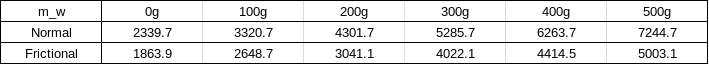
\includegraphics[scale=0.75]{GraphStatic1.png} \\ \\ 
        {\large Experiment for computing $\mu_k$ on rough sandpaper surface } \\
        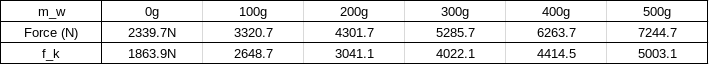
\includegraphics[scale=0.75 ]{GraphKinetic1.png} \\ \\
        {\large Mass vs Normal Force and Frictional Force for sandpaper} \\ 
        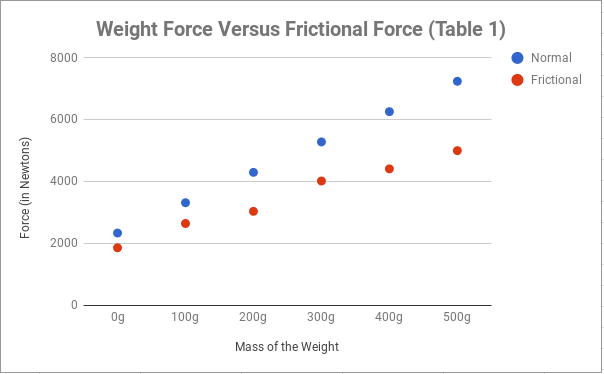
\includegraphics[scale=0.75]{GraphWeightVsFriction1.png} \\ \\
        {\large Experiment for computing $\mu_k$ on smoother wooden surface} \\
        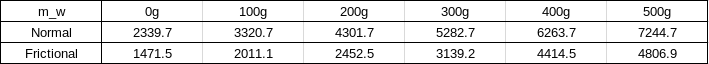
\includegraphics[width=\textwidth]{GraphKinetic2.png} \\ \\
        {\large Mass vs Normal Force and Frictional Force for wood} \\ 
        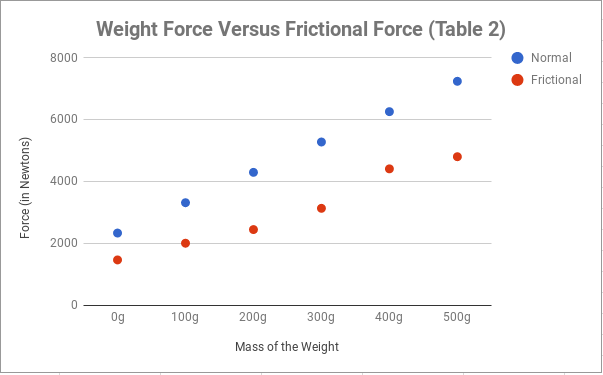
\includegraphics[scale=0.75]{GraphWeightVsFriction2.png} \\ \\
        {\large Experiment for determining sliding angle and $\mu_s$} \\
        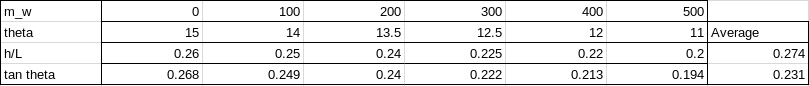
\includegraphics[scale=0.6]{DataTable3.png} \\ \\


    \section{Analysis}
        \subsection{Equations}
            \par To determine $\mu_s$, we use the scenario where the force of
            gravity on the hanging weight equals the pulling force of the
            block plus the friction acting against the weight pulling down.
            The sloped force of the block without friction can be represented
            as
            \begin{equation}
                F_{\parallel} = F_g * \sin{\theta}
            \end{equation}
            Where $F_{\parallel}$ is the parallel force of the weight, $F_g$
            is the force of gravity of the block (equal to $m_{block}g$) and
            $\theta$ is the incline's angle of elevation.

            \par The force of friction will be directed in the same direction
            as $F_{\parallel}$, and it can be expressed as
            \begin{equation}
                F_k = F_n * \mu_k
            \end{equation}
            \begin{equation}
                F_s = F_n * \mu_s
            \end{equation}
            Where $F_k$ and $F_s$ are the forces of kinetic and static friction
            respectively, $F_n$ is the normal force of the block on the slope,
            and $\mu_k$ and $\mu_s$ are the coefficients of kinetic and static
            friction respectively. $F_n$ can be rewritten as $F_{\bot}$
            as the normal force is the perpendicular force enacted by the slope
            on the block. This normal force can be written as $F_g *\cos{\theta}$
            The force of gravity on the hanhging weight can be represented as
            \begin{equation}
                F_{gw} = m_w * g
            \end{equation}
            \par In our experiment, $F_{\parallel}$ combined with $F_k$ or $F_s$
            are equal to $F_{gw}$ which lets us iscolate for $\mu_s$.
    \section{Conclusion}
        Our data gave us a relatively consistent reading on $\mu_k$ and $\mu_s$ which
        indicates that the fundamental laws of physics that are well understood
        and accepted as fact are, surprisingly, accurate. Our deviation of $\mu_k$
        gives us a possible error of around 5\%, and our deviation of $\mu_s$ gives
        us an error of about 7\%. This error could have been caused by the tape
        markings on the platform that the blocks slid over, and it can also be
        caused by friction in the pulley that we used to measure the force of the
        sliding masses.
\end{document}
